\section{Flow of Data}
\subsection{Characteristics}
\begin{itemize}
	\item Bandwidth: The volume of data per second, or bits per second. (eg. 40 Gbps capacity is 40 Gigabit per second)
	\item Latency: The time it takes for a particular bit or group of bits to travel through a network. Limited by speed of light.
	\item Error Rate: Can be caused by anything (cosmic rays, cable issues, etc.). Determines how much error checking and correction is justifiable.
\end{itemize}
\paragraph{Trade-Off Data}
Different applications have different requirements because we don't live in an ideal world. Voice programs can accept low bandwidth and high errors, but latency problems are a big no no. File transfer of operating system images is mostly concerned with reliability; you don't want a corrupted OS. The trade-offs are dependent on the application, so anything from speed, error or latency can be traded off for your desire purpose.
\paragraph{Circuit Switching}
Old phones were linked with physical wires, so the phone on one end was continuously connected to the speaker on other end. This was very inefficient; even if no audio was being transferred the line would be reserved. Multiplexing was very complicated and expensive using 1950s tech, so circuit switching was not a good method for networking. We can use packet switching in a circuit.
   \begin{figure}[!htb]
	\center{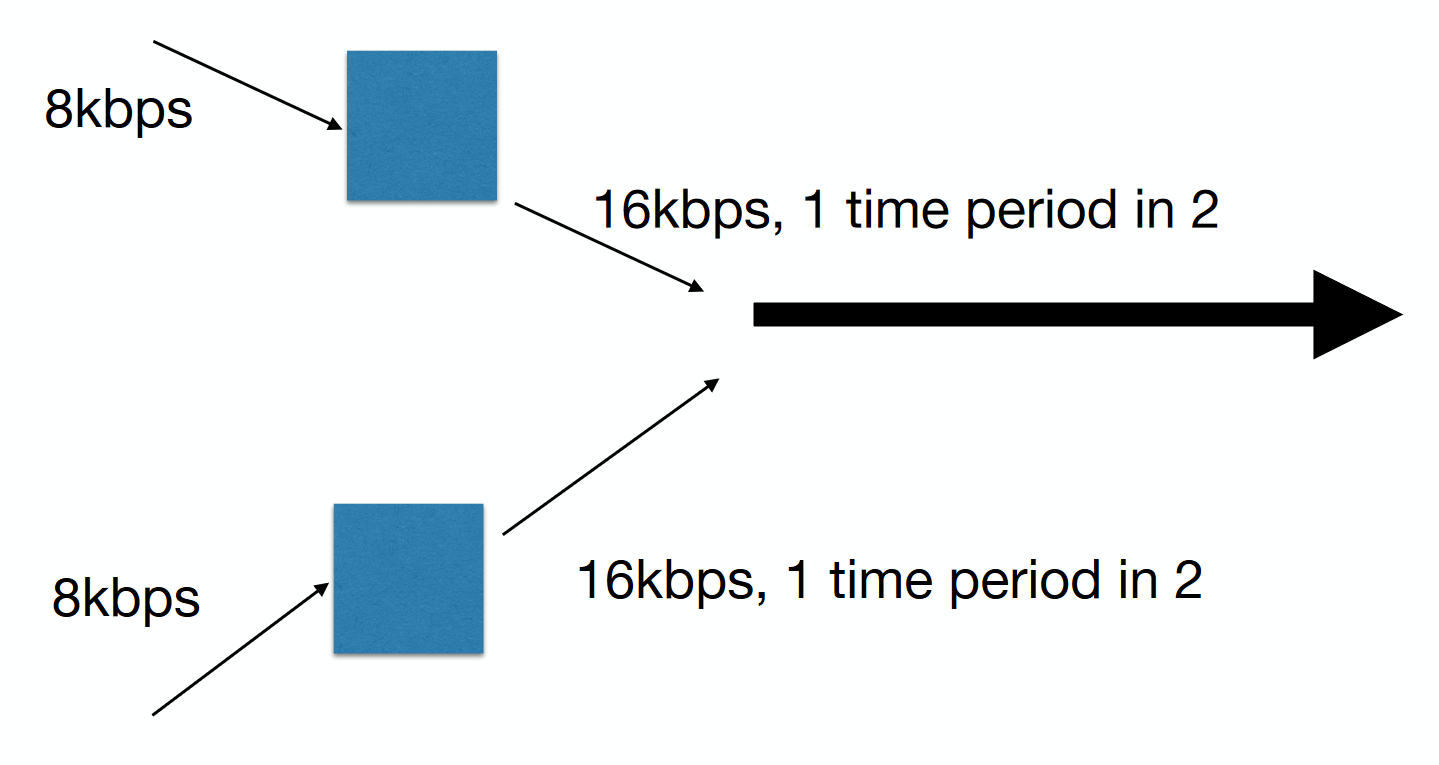
\includegraphics[width=9cm]
		{networks/packetswitching}}
	\caption{\label{fig:packetswitching} Packet switching in Time domain with 8 kbps lines into a 16 kbps line}
\end{figure}
\paragraph{Packet Switching}
Instead of having a continuous stream of data, we can divide it into smaller units called "packets". We can use these packets and switch them across the network to reach their destination. By splitting them into smaller units, you can multiplex the packets in the time domain, instead of the frequency domain. It is easier to build, but adds latency. You end up with a statistical gain in bandwidth because no resources are used while no data is being sent.
\paragraph{Virtual Circuits}
Virtual circuits aim to emulate physical circuits. Endpoints tell the network to establish a connection between them; this path is then given an identifier used throughout the network to route the emulated connections. Once A connection is no longer needed, it is "torn down" like a physical circuit. This method allows the network to know everything happening with the connection, and could be used to sort out packet issues. The finer details are removed from the end user with virtual circuits.
\paragraph{Datagrams}
Packets in the datagram method contain complete address information. There is no line connecting two endpoints, instead packets are sent off on a journey through the network space. All that happens is the network routes the packets using the data in the packet. All implementation and packet issues are dealt with at the endpoints. This is referred to as a datagram service.
\subsection{Layering}
A way to think of networks as having different layers of interactions. Each layer provides a service to those above it and makes use of services to those below it. There are two major models we looked at, OSI (a failure) and DOD (a success). We will focus on DoD as it is used everywhere.
   \begin{figure}[!htb]
	\center{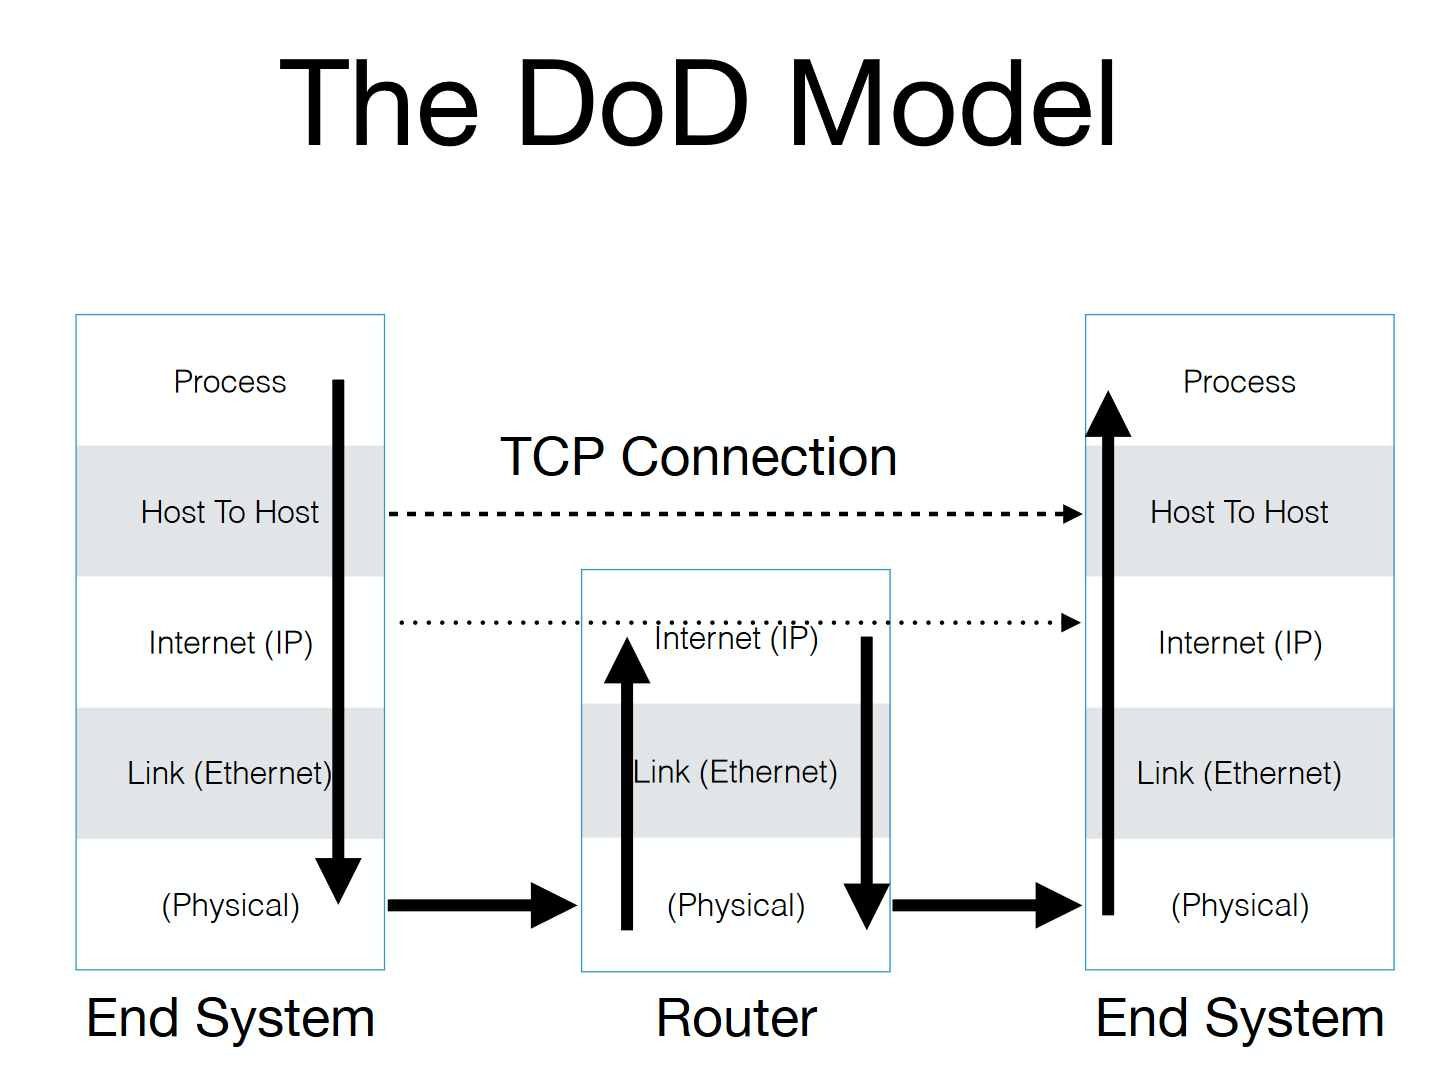
\includegraphics[width=11cm]
		{networks/dodmodel}}
	\caption{\label{fig:dodmodel} End-to-End DoD Model}
\end{figure}
\paragraph{Process}
Processes or Applications are running code that do actual work, and the protocols they use. (eg. HTTP, ssh)
\paragraph{Host-to-Host}
Host-to-Host transport layer moves data between two end systems via a network whose topology and other properties the transport layer doesn't know much about. (TCP for streams, UDP for packets). This layer guarantees various properties; reliability, sequenced delivery, etc. This layer also deals with separating data between the appropriate applications.
\paragraph{IP}
This layer moves packets between end systems, but doesn't offer any guarantees. It handles choosing which link to get the data closer to its destination. This layer does not deal with separating data by applications. Uses IPv4/IPv6.
\paragraph{Link}
This layer moves data between one network element and the next element; concerned with packetisation, addressing, etc. Can have a variety of protocols in use (Ethernet primarily, ATM sometimes pops up)
\paragraph{Physical}
The physical layer is the actual encoding used to shift bits over a distance. (eg. Fibre Optics)
   \begin{figure}[!htb]
	\center{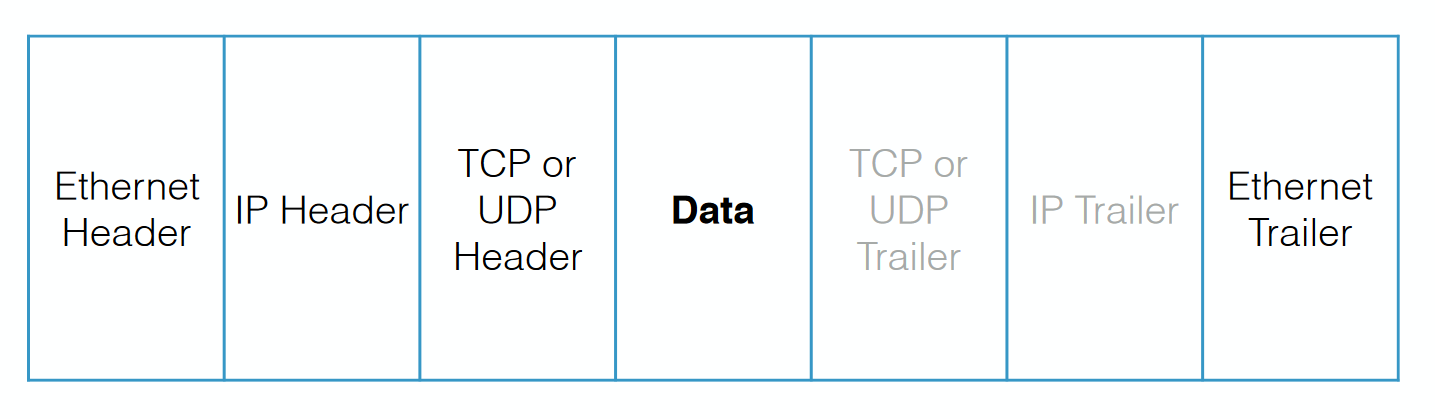
\includegraphics[width=13cm]
		{networks/packet}}
	\caption{\label{fig:packet} Layers encapsulated by packet structure}
\end{figure}

\subsection{Ethernet}
Network spaces can be divided as Local Area Networks (LAN), Wide Area Networks (WAN) WAN technology through most of its history was slow and unreliable. In terms of the lowest layer of networking, Ethernet is the most widely used. Ethernet was originally a bus; a single cable with computers connected throughout it. Packets were transferred through the cable; minimum size 64 bytes.
\paragraph{Ethernet}
The first set of bits on an ethernet cable is composed of alternating 1 and 0; this is because the clocks of computers can be horribly desynced (+- 50ppm), so the stream of 1 and 0 was used for clock syncing. There is also a method of calculating checksums continuously to find the end of a packet instead of just an end buffer. Ethernet's main issue is network collisions.
\paragraph{Collision Detection}
Ethernet is formally known as "CSMA CD" - Carrier Sense Multiple Access Collision Detection. Systems connected to Ethernet effectively share a line, each system reserving it while sending data. If more than one device is transmitting at a time, this results in packet collisions and causes packets to get corrupted. Collision is detected by the transmitted also listening on the cable; if there is a mismatch, collision detected. The system then sends a jamming signal alerting of a collision. The minimum packet size exists to ensure collisions are detected in the cable due to latency.
\paragraph{Recovery}
On the nth attempt of collision recovery, the system chooses a random number k from ${0..2^k}$ and delay k x 512 bit periods before trying again. After 10 attempts it simply gives up. Random generation isn't anything fancy, so long as its generation is different from other systems in the cluster.
\paragraph{Problems}
Collisions increase non-linearly with load, and the precise curve depends on the exact traffic mix. This sharp increase meant that adding more systems crippled performance. Latency was also unpredictable due to the collision system using random values, meaning it's impossible to be specific about latency.
\paragraph{Cables}
\begin{itemize}
	\item 10base5: 500m length cables with speed 10 MBps; heavy coax cables, expensive, difficult to work with
	\item 10base2: Thing coax, higher resistance but 185m length, instead of transceivers, simply T-piece
	\item 10baseT: Modern ethernet, modem internet, uses RJ45 connectors to a hub, originally Cat3 cables (think phone cables can now be used for networking)
\end{itemize}
   \begin{figure}[!htb]
	\center{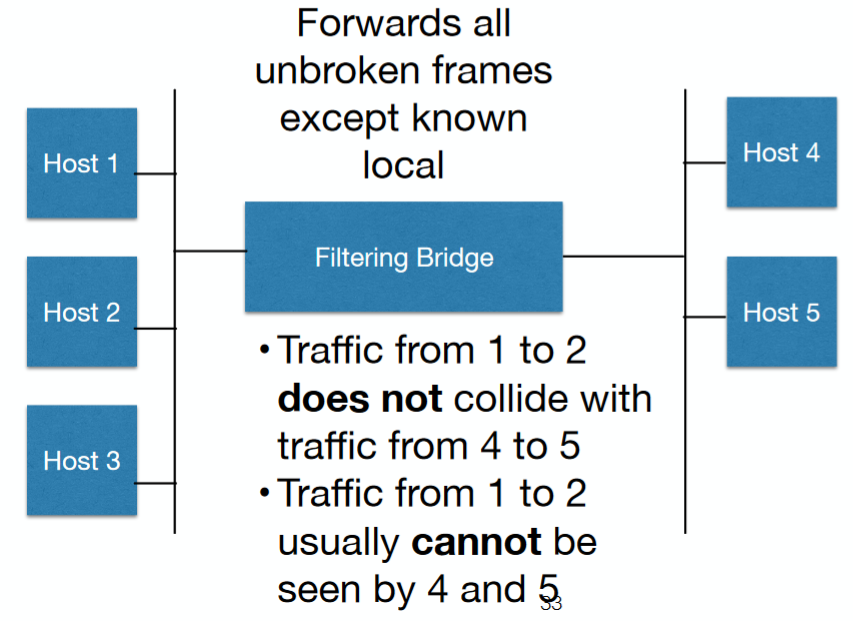
\includegraphics[width=9cm]
		{networks/smartbridge}}
	\caption{\label{fig:smartbridge} Smart bridges increased network speed by allowing connections in different clusters to simultaneously function without interrupting each other}
\end{figure}
\paragraph{Ethernet Add-ons}
\begin{itemize}
	\item Repeater: An analogue amplifier, collisions can be seen on both sides
	\item (Smart) Bridge: Receives, buffers and transmits frames, so collisions are not propagated
	\item (Dumb) Bridge: Propagates everything, regardless of source and destination address being on one side
\end{itemize}
